\section{Methodology}
\label{sec:method}

\subsection{Overview}
We adopt the representation-based approach introduced in Section~\ref{sec:intro}: an encoder first learns speech representations from unlabeled Thai audio, and the same encoder is then adapted to transcription using a limited amount of labeled speech. Fig.~\ref{fig:framework} summarizes the two stages. In Stage~1 (pretraining), log-Mel features computed from untranscribed Thai recordings are passed to a speech-adapted Audio-JEPA, which learns by predicting the latent features of hidden time spans \cite{tuncay2025audiojepa}. In Stage~2 (fine-tuning), the pretrained context encoder is transferred to a recognizer, a connectionist temporal classification (CTC) head \cite{graves2006ctc} is attached, and the model is trained on Thai transcripts under fixed labeled-data budgets. The JEPA predictor and target encoder are discarded after Stage~1, so they add no inference cost.

\begin{figure*}[t]
\centering
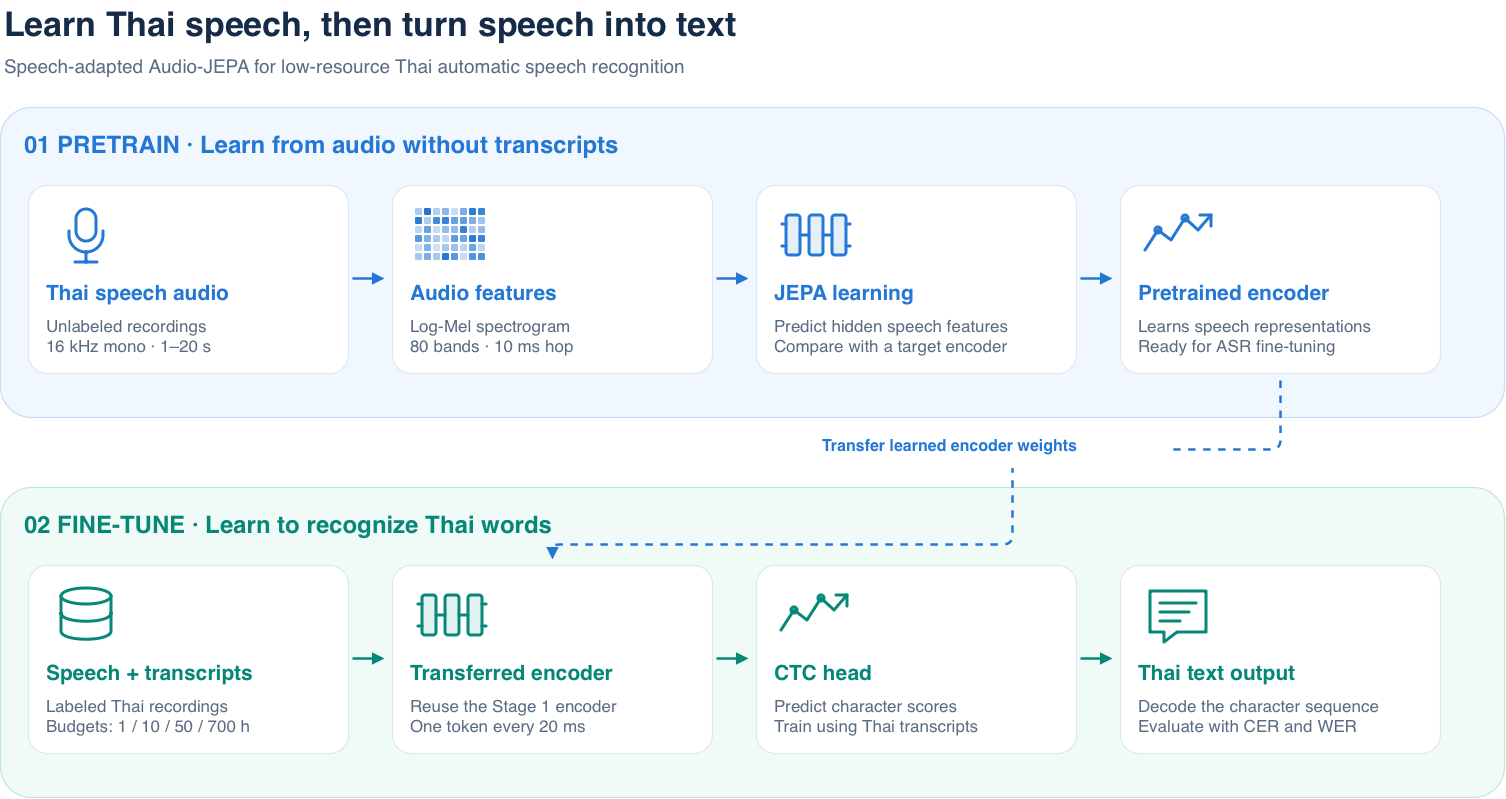
\includegraphics[width=\textwidth]{figures/framework_overview.png}
\caption{Overall framework. Stage~1 pretrains a speech-adapted Audio-JEPA encoder on unlabeled Thai audio. Stage~2 transfers the learned encoder weights to a CTC recognizer trained with 1, 10, 50, or approximately 700 hours of transcribed Thai speech and evaluated with CER and WER.}
\label{fig:framework}
\end{figure*}

\subsection{Dataset and Text Processing}
\label{sec:data}
Experiments use the Porjai Central Thai speech corpus released by CMKL \cite{porjai}. Because the corpus does not provide speaker identifiers, utterances are assigned to training, validation, and test partitions (80\%/10\%/10\%) by a deterministic hash of the utterance identifier. Every run therefore uses identical partitions. A consequence is that the partitions are utterance-disjoint but not guaranteed to be speaker-disjoint; we treat this as a limitation when interpreting test results. Self-supervised pretraining reads audio only from the training partition. Validation and test audio is never seen during Stage~1, and transcripts are never seen in Stage~1 at all.

Audio is decoded, converted to mono, and resampled to 16~kHz. Utterances outside the permitted duration range are removed from training instead of being truncated, so every training waveform remains consistent with its full transcript. The number of excluded utterances and hours is logged for each run.

Transcripts are normalized with a single rule set that is applied identically to training labels, references, and hypotheses: Unicode NFKC normalization, removal of zero-width characters and punctuation, mapping of Thai digits to Arabic digits, lowercasing of Latin letters, and collapsing of repeated whitespace. Thai vowels, tone marks, and the repetition mark are retained. The output vocabulary is character-level and includes Thai consonants, vowels, tone and orthographic marks, digits, Latin letters, a word-boundary space token, an unknown token, and the CTC blank at index~0. Characters outside the vocabulary map to the unknown token during training, but references keep their original characters, so such characters still count as errors at evaluation.

\subsection{Acoustic Frontend and Speech Tokenization}
\label{sec:frontend}
Each waveform is converted to 80 log-Mel filterbank features using a 25~ms analysis window and a 10~ms hop. The original Audio-JEPA divides a $256\times128$ spectrogram into $16\times16$ patches, which yields only 16 temporal positions for a 10-second clip, or one position every 625~ms \cite{tuncay2025audiojepa}. CTC requires that the number of output frames $T$ satisfies
\begin{equation}
T \ge U + R,
\label{eq:ctcfeas}
\end{equation}
where $U$ is the transcript length and $R$ is the number of adjacent repeated labels, because repeated labels must be separated by a blank. A character-level Thai transcript typically has more characters than the coarse grid has time steps, so most utterances cannot be aligned at that resolution.

We therefore replace the square patch embedding with a full-frequency temporal projection stem. A two-dimensional convolution with kernel and stride $(80,2)$ and 768 output channels maps each pair of consecutive 10~ms frames, across all 80 Mel bands, to one 768-dimensional token. The encoder thus receives one token every 20~ms (50 tokens per second), as shown in Fig.~\ref{fig:jepa}. The exact number of valid tokens is computed from the unpadded waveform length:
\begin{equation}
F=\left\lfloor\frac{N-W}{H}\right\rfloor+1,\qquad
T=\left\lfloor\frac{F-2}{2}\right\rfloor+1,
\end{equation}
where $N$ is the number of samples, $W$ and $H$ are the window and hop lengths in samples, $F$ is the number of filterbank frames, and $T$ is the number of encoder tokens. These valid lengths, rather than padded tensor lengths, define the attention masks, the masking region in Stage~1, and the CTC input lengths in Stage~2. Before training, every batch is checked against \eqref{eq:ctcfeas}, and the ratio $T/(U+R)$ is reported.

\subsection{Encoder Architecture}
The encoder keeps the Audio-JEPA Vision Transformer backbone: 12 pre-LayerNorm Transformer blocks with width 768, 12 attention heads, and a feed-forward width of 3072 with GELU activations, followed by a final LayerNorm \cite{tuncay2025audiojepa}. Fixed sinusoidal positional embeddings are added to the tokens along the time axis. Padded positions are excluded from self-attention by an additive attention mask. The encoder has no classification token and performs no temporal pooling, so its output is an ordered sequence of 20~ms frame representations. The model attends bidirectionally and targets offline transcription.

\subsection{Stage 1: Thai Speech JEPA Pretraining}
\label{sec:ssl}

\begin{figure*}[t]
\centering
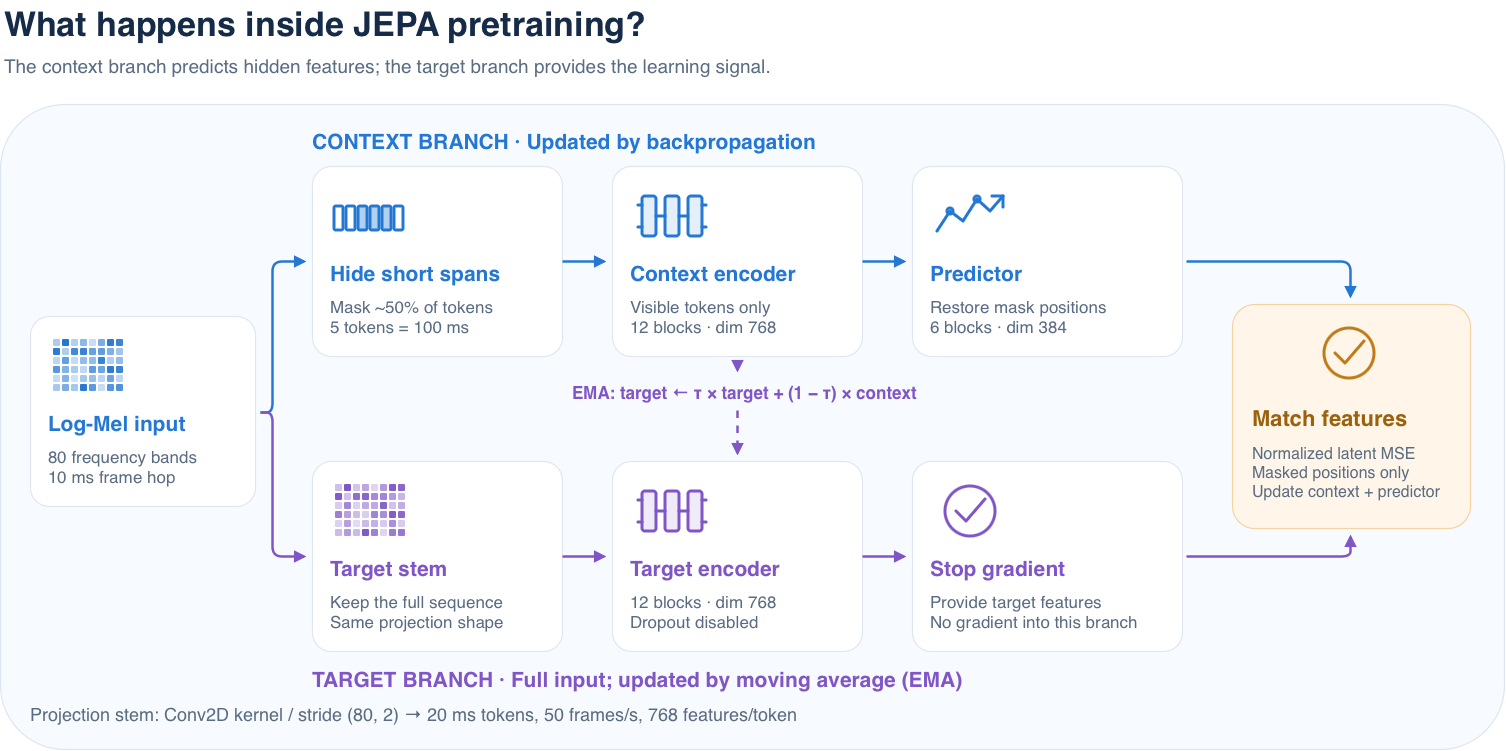
\includegraphics[width=\textwidth]{figures/jepa_learning.png}
\caption{Inside JEPA pretraining. The context branch sees only visible tokens and predicts latent features at the hidden positions. The target branch encodes the complete sequence and provides stop-gradient targets. Gradients update the context stem, context encoder, and predictor. The target branch is updated only by an exponential moving average (EMA) of the context weights.}
\label{fig:jepa}
\end{figure*}

Fig.~\ref{fig:jepa} details the pretraining objective. Let $P_\theta$ denote the projection stem and $E_\theta$ the context encoder. A target copy $(P_{\bar\theta},E_{\bar\theta})$ is initialized with identical weights and receives no gradients.

\subsubsection{Short-span temporal masking}
The original Audio-JEPA samples random two-dimensional blocks on the spectrogram patch grid \cite{tuncay2025audiojepa}. Speech information is organized mainly along time, so we mask whole time steps across all frequencies. For each batch, spans of five consecutive tokens (100~ms, roughly phone-to-syllable scale) are sampled within the valid region until approximately 50\% of the valid tokens are hidden. The context branch receives only the remaining visible tokens, each with its original positional embedding. Prediction targets are drawn from the hidden spans, with two target sets per batch. Padding is never selected as context or target. Hiding short spans prevents the model from solving the task by copying immediately adjacent frames, while leaving enough surrounding context to infer the hidden content.

\subsubsection{Predictor}
The predictor is a narrower Transformer with 6 blocks of width 384 and 12 heads. Context outputs are linearly projected to width 384. A shared learnable mask token, plus the positional embedding of each hidden position, is appended for every target position, and the sequence is processed by the predictor blocks. A final linear layer maps the outputs back to 768 dimensions, giving the prediction $\hat z_t$ for each target position $t$.

\subsubsection{Latent prediction objective}
Let $z_t$ be the target encoder output at position $t$, and let $\bar z_t$ be $z_t$ standardized across its channels. Following the normalized latent loss of Audio-JEPA, we minimize the squared distance between $\ell_2$-normalized prediction and target vectors over the set of target positions $M$:
\begin{equation}
\begin{aligned}
\mathcal{L}_{\mathrm{JEPA}}
&=\frac{1}{|M|}\sum_{t\in M}
\left\|\frac{\hat z_t}{\|\hat z_t\|_2}-
\operatorname{sg}\!\left[\frac{\bar z_t}{\|\bar z_t\|_2}\right]\right\|_2^2\\
&=\frac{1}{|M|}\sum_{t\in M}\bigl(2-2\cos(\hat z_t,\bar z_t)\bigr),
\end{aligned}
\label{eq:jepa}
\end{equation}
where $\operatorname{sg}[\cdot]$ stops gradients. The loss is computed only at hidden positions and is averaged over the target sets. Because the targets are features rather than spectrogram values, the model is not required to reproduce low-level acoustic detail such as background noise.

\subsubsection{EMA target update}
Only the context stem, context encoder, and predictor are optimized. After each update, the target parameters follow an exponential moving average of the context parameters:
\begin{equation}
\bar\theta\leftarrow\tau_s\bar\theta+(1-\tau_s)\theta,\qquad
\tau_s=1-(1-\tau_0)\,\frac{1+\cos(\pi s/S)}{2},
\end{equation}
with $\tau_0=0.996$, so $\tau_s$ rises from 0.996 to 1.0 over the $S$ pretraining updates. Dropout is disabled in the target branch.

\subsubsection{Collapse monitoring}
Latent prediction objectives admit a trivial solution in which all embeddings become constant. The EMA target and stop-gradient discourage this solution but do not rule it out. During pretraining we therefore log the per-channel variance of target features, the mean cosine similarity between utterance-level embeddings within a batch, and the mean feature norm. A run whose loss falls while feature variance approaches zero or inter-utterance similarity approaches one is treated as collapsed and is not used for fine-tuning.

\subsubsection{Initialization}
Stage~1 is run from two initializations. In the transfer setting, all Transformer blocks and the final LayerNorm are loaded from the public Audio-JEPA checkpoint pretrained on AudioSet \cite{tuncay2025audiojepa,audiojepacode}. The projection stem cannot be loaded because its kernel shape differs from the original $16\times16$ patch embedding, so it is initialized randomly. The pretraining then continues on Thai audio. In the scratch setting, all weights are initialized randomly. A loading report records every loaded, reinitialized, and skipped tensor together with the fraction of parameters transferred.

\subsection{Stage 2: CTC Fine-Tuning}
\label{sec:ctc}
After pretraining, the context stem and context encoder are kept. The predictor and target branch are removed. A dropout layer ($p=0.1$) and a linear layer map each 768-dimensional frame representation to a distribution over the vocabulary $\mathcal{V}$ and the blank symbol $\varnothing$. For an input $x$ with transcript $y$, training minimizes the CTC loss
\begin{equation}
\mathcal{L}_{\mathrm{CTC}}=-\log\sum_{\pi\in\mathcal{B}^{-1}(y)}\prod_{t=1}^{T}p(\pi_t\mid x),
\end{equation}
where $\mathcal{B}$ merges consecutive identical labels and then removes blanks \cite{graves2006ctc}. Input lengths are the valid token counts defined in Section~\ref{sec:frontend}. Infinite losses are not replaced with zero, so any alignment failure is visible in the logs.

Because the projection stem has been retrained or newly initialized, the optimizer uses three parameter groups with separate learning rates: the Transformer backbone, the projection stem, and the CTC head. Pretrained backbones use a learning rate one-tenth of the head learning rate, whereas the stem and head use larger rates. When a frozen-encoder variant is run, only the Transformer blocks are frozen, and the stem and head remain trainable. Inference uses greedy CTC decoding: the most probable label is selected at each valid frame, repeats are merged, and blanks are removed. No external language model is used.

\subsection{Experimental Configurations}
\label{sec:configs}
Table~\ref{tab:configs} lists the systems. All systems share the same frontend, partitions, vocabulary, CTC head, and decoding procedure. Comparing them isolates three factors: the value of upstream Audio-JEPA weights (A versus B), the value of in-domain Thai JEPA pretraining (B versus C), and whether Thai JEPA pretraining alone, without AudioSet weights, is sufficient (A versus D). A wav2vec~2.0 encoder fine-tuned with an identical CTC head serves as a speech-specialized self-supervised reference \cite{baevski2020wav2vec2}. Its pretraining data and model size differ from those of our encoder, so it is a practical reference point rather than a controlled comparison of objectives.

\begin{table}[t]
\caption{Experimental configurations. All systems end with a newly initialized CTC head.}
\label{tab:configs}
\centering\footnotesize
\begin{tabularx}{\columnwidth}{@{}l l X@{}}
\toprule
ID & Encoder initialization & Purpose \\
\midrule
A & Random & Supervised-only control \\
B & Audio-JEPA (AudioSet) & Effect of upstream transfer \\
C & Audio-JEPA $\rightarrow$ Thai JEPA & Effect of in-domain Thai pretraining (proposed) \\
D & Random $\rightarrow$ Thai JEPA & Thai pretraining without AudioSet weights \\
Ref & wav2vec~2.0 & Speech-specialized SSL reference \\
\bottomrule
\end{tabularx}
\end{table}

To measure label efficiency, CTC fine-tuning is repeated with nested labeled subsets of 1, 10, and 50 hours and with the full training partition of approximately 700 hours. Each smaller subset is contained in every larger one. Self-supervised pretraining always uses the same unlabeled training audio, so only the transcription budget varies across conditions. Each configuration is trained with three random seeds (42, 43, and 44), and results are reported as mean $\pm$ standard deviation.

\subsection{Training Details}
Table~\ref{tab:hparams} lists the optimization settings, taken from the experiment configurations in our codebase. Both stages use AdamW with a linear warmup over the first 10\% of updates, followed by cosine decay to 1\% of the peak learning rate, and gradient clipping at norm~1.0. Weight decay is not applied to biases or normalization parameters. The checkpoint with the lowest validation CER is selected, and training stops early when validation CER stops improving.

\begin{table}[t]
\caption{Optimization settings for both training stages.}
\label{tab:hparams}
\centering\footnotesize
\begin{tabularx}{\columnwidth}{@{}p{0.32\columnwidth} X@{}}
\toprule
Setting & Value \\
\midrule
\multicolumn{2}{@{}l}{\textit{Stage 1: JEPA pretraining}} \\
Optimizer & AdamW, learning rate $1\times10^{-4}$, weight decay 0.01 \\
Batch / epochs & 8 utterances per batch; 8 epochs \\
Masking & 5-token (100~ms) spans, about 50\% of valid tokens; 2 target sets \\
Predictor & 6 blocks, width 384, 12 heads \\
EMA & $\tau$: 0.996 $\rightarrow$ 1.0, cosine schedule \\
\midrule
\multicolumn{2}{@{}l}{\textit{Stage 2: CTC fine-tuning}} \\
Learning rates & Head $3\times10^{-4}$; stem $3\times10^{-4}$ ($1\times10^{-4}$ after Thai JEPA); backbone $3\times10^{-5}$ if pretrained, $3\times10^{-4}$ if random \\
Batch / epochs & 8 utterances, up to 15 epochs (1~h budget: 4 utterances, up to 25 epochs) \\
Early stopping & Patience of 5 validation evaluations (8 for the 1~h budget) \\
Regularization & Dropout 0.1 before the CTC head; weight decay 0.01 \\
Decoding & Greedy CTC, no language model \\
\bottomrule
\end{tabularx}
\end{table}

\subsection{Evaluation Metrics}
\label{sec:metrics}
The primary metric is the character error rate (CER). Because Thai is written without spaces between words, word error rate (WER) requires word segmentation. We segment both references and hypotheses with the PyThaiNLP \texttt{newmm} dictionary-based tokenizer \cite{pythainlp}, with the same version and dictionary for all systems, and then compute WER. For both units,
\begin{equation}
\mathrm{ER}=\frac{S+D+I}{N}\times100\%,
\end{equation}
where $S$, $D$, and $I$ are the numbers of substitutions, deletions, and insertions, and $N$ is the number of reference units. Counts are accumulated over the whole evaluation set rather than averaged per utterance. Model selection uses only the validation partition. The test partition is evaluated once, with the selected checkpoint of each run.
